\begin{figure}[!ht]
    \centering
        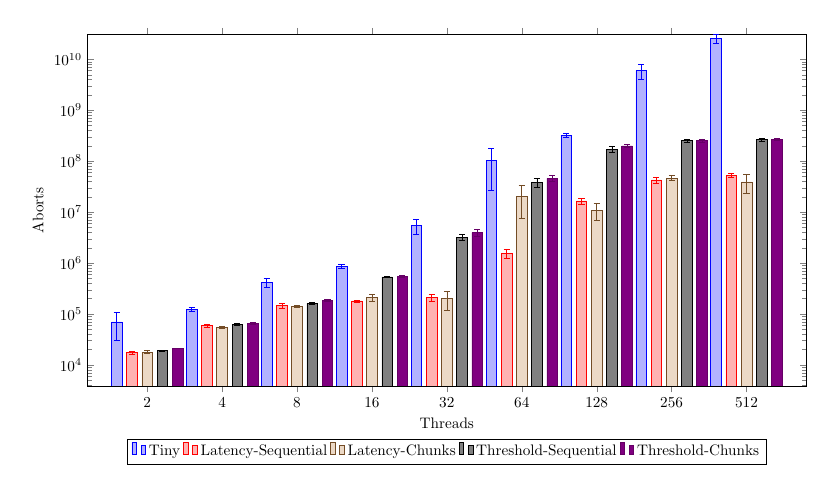
\begin{tikzpicture}[scale=0.55, baseline]
        \begin{axis}[
            ymode=log,
            width=1.5 \linewidth,
            height=0.8 \linewidth,
            %media de tempo intruder
            ybar=3pt,
            %enlargelimits=0.10,
            legend style={at={(0.5,-0.15)}, anchor=north, legend columns=-1},
            ylabel=Aborts,
            xlabel=Threads,
            symbolic x coords={1, 2, 4, 8, 16, 32, 64, 128, 256, 512},
            xtick=data,
            ymin=0,
            ymax=31000000000,
            bar width=7pt,
            % nodes near coords,
            nodes near coords align={vertical},
        ]
        \addplot+[error bars,y dir=both, y explicit] coordinates {
            (1,0.0)+-(1,0.0) (2,69940.4)+-(2,38859.442881235445) (4,123224.4)+-(4,10230.047558051723) (8,421702.0)+-(8,83144.47432752221) (16,858817.0)+-(16,70319.27963794851) (32,5482927.6)+-(32,1822574.306164838) (64,102125071.2)+-(64,75531726.60526115) (128,324906951.0)+-(128,25833176.356745664) (256,5976414236.0)+-(256,1965369780.1742249) (512,25331573456.2)+-(512,5125278647.27645) 
        };
        \addplot+[error bars,y dir=both, y explicit] coordinates {
            (1,0.0)+-(1,0.0) (2,17295.8)+-(2,884.117051074121) (4,58832.4)+-(4,5182.0950049183775) (8,145328.0)+-(8,14502.15570182585) (16,179942.6)+-(16,9939.803108713975) (32,213282.4)+-(32,33756.78063204487) (64,1563534.8)+-(64,303501.08637854987) (128,16550448.4)+-(128,2123035.5644618487) (256,42956098.2)+-(256,6012180.935710481) (512,52269879.0)+-(512,4755551.76397057)
        };
        \addplot+[error bars,y dir=both, y explicit] coordinates {
             (1,0.0)+-(1,0.0) (2,17786.7)+-(2,1249.259304548099) (4,54750.2)+-(4,2738.370420523856) (8,141273.5)+-(8,6123.819286197136) (16,209526.5)+-(16,34736.26421551402) (32,201599.3)+-(32,81127.76465680539) (64,20569626.4)+-(64,12875680.754533986) (128,10897558.0)+-(128,4040389.7657925775) (256,46668204.777777776)+-(256,5450523.901092766) (512,39389491.0)+-(512,16022591.920577014) 
        };
        \addplot+[error bars,y dir=both, y explicit] coordinates {
            (1,0.0)+-(1,0.0) (2,19074.2)+-(2,369.0059078117856) (4,61648.4)+-(4,2902.3763091646124) (8,161693.8)+-(8,9525.331540686655) (16,536547.4)+-(16,18869.180433712536) (32,3237316.8)+-(32,385306.9331768636) (64,38103581.6)+-(64,7477543.014654762) (128,171013189.4)+-(128,21848968.54501459) (256,256035773.6)+-(256,17482704.25370147) (512,263634097.2)+-(512,12981014.911830684)
        };
        \addplot+[error bars,y dir=both, y explicit] coordinates {
            (1,0.0)+-(1,0.0) (2,21093.1)+-(2,312.0) (4,64726.72)+-(4,3041.77) (8,183647.1)+-(8,8673.62) (16,544787.54)+-(16,23782.8) (32,3980021.4)+-(32,552484.0028907986) (64,45836278.2)+-(64,6287845.41) (128,199521897.4)+-(128,10431600.060439752) (256,254781534.6)+-(256,19017136.502195936) (512,266950650.75)+-(512,14874593.300939599)
        };
        \legend {Tiny, Latency-Sequential, Latency-Chunks, Threshold-Sequential, Threshold-Chunks}
        \end{axis}
        \end{tikzpicture}
    \caption{Aborts do benchmark Vacation variando o número de \emph{threads}.}
    \label{vacation_abort}

\end{figure}